\documentclass[letterpaper, 10 pt, conference]{../ieeeconf} 
\IEEEoverridecommandlockouts
\overrideIEEEmargins
\pdfoptionpdfminorversion=4

\usepackage{amsmath}
\usepackage{mathtools}
\usepackage{textcomp}
\usepackage{graphicx}
\usepackage[font=footnotesize]{subcaption}
\usepackage[font=footnotesize]{caption}
\usepackage{hyperref}
\usepackage{amssymb}
\usepackage{booktabs}
\usepackage[normalem]{ulem}
\usepackage{verbatim}
\usepackage[export]{adjustbox}
\usepackage{amsmath}
\usepackage{url}
\usepackage{siunitx}
\usepackage[utf8]{inputenc}
\usepackage[TS1,T1]{fontenc}
\usepackage{array, booktabs}
\usepackage{caption}
\usepackage[cal=cm]{mathalfa}
\usepackage{algorithm}
\usepackage[noend]{algpseudocode}

% Labels in IEEE format
\newcommand{\eref}[1]{(\ref{#1})} % Equation
\newcommand{\sref}[1]{Sec.~\ref{#1}} % Section
\newcommand{\figref}[1]{Fig.~\ref{#1}} % Figure
\newcommand{\tref}[1]{Table~\ref{#1}} % Table
\newcommand{\aref}[1]{Algorithm~\ref{#1}} % Algorithm
\newcommand{\lref}[1]{Line~\ref{#1}} % Line
\renewcommand*\rmdefault{ppl}
\setlength{\textfloatsep}{5pt}

\usepackage{ifthen}
\usepackage[usenames,dvipsnames,table]{xcolor}
\newboolean{include-notes}
\setboolean{include-notes}{true} 
% http://en.wikibooks.org/wiki/LaTeX/Colors
\newcommand{\rhnote}[1]{\ifthenelse{\boolean{include-notes}}%
 {\textcolor{blue}{\textbf{RH: #1}}}{}}
\newcommand{\sanote}[1]{\ifthenelse{\boolean{include-notes}}%
 {\textcolor{green}{\textbf{SAN: #1}}}{}}

\begin{document}

% paper title
\title{6.857 Final Project: Milestone 5}
\author{Sebastiani Aguirre Navarro and Rachel Holladay}
\maketitle

\section{Introduction}
Our goal is to use neural networks to classify whether a particular grasp will succeed on an object.
We utilize the Dexerity Network (DexNet) 2.0 data set~\cite{mahler2017dex}, that has 6.7 million synthetic point clouds with parallel-jaw grasps (a common robot hand type of two parallel fingers) and analytical grasp metrics.
The authors of the data set trained a Grasp Quality Convolutional Neural Network (GQ-CNN), which achieved 85.7\% accuracy on their classification task.
To accomplish the same task, we will be experimenting with new architectures, intput formats, other modifications described in~\sref{sec:questions}.
Most of the recent machine learning papers in robotics present a problem, dataset and, usually, an optimized convolutional neural network with some architecture and input format. 
Our goal is to explore the process of finding that CNN and exploring the factors that effect performance. 
While our results will only be verified according to this data set, and therefore cannot be generalized to all CNNs, we hope to gain intution, understanding, and, hopefully, a higher accuracy. 
Having explored various components, we will optimize our final, best architecture. 

We will first describe the data set generation process and the features provided in the data set~\sref{sec:data_set}. 
Understanding and processing this data set has become a larger element of our project then previously anticipated. 
We next discuss our results thus far~\sref{sec:results}, which are preliminary. 
We will continue to explore these results, as well as our research questions~\sref{sec:questions}. 


\section{Data Set}
\label{sec:data_set}
We are using the Dex Net 2.0 data set as first presented in~\cite{mahler2017dex}. 
We first briefly summarize their data generation process before describing how we manipulated the data. 

Mahler et al define a generative graphical model defined over the camera pose, object shape and pose, friction coeffient, grasp, depth image and success metric. 
To generate the data set they make i.i.d (independent and identically distributed) samples from their generative graphical model, resulting in 6.7 million data points. 

The data set is defined over 1,500 object meshes that were used in Dex-Net 1.0~\cite{mahler2016dex}, collected from a variety of other data bases and standardized with respect to position.
For each object, they generated 100 parallel jaw grasps via rejection sampling of antipodal pairs and evaluated a grasp metric on each grasp. 
Additionally, each object is paired with a rendered depth image (2.5D point cloud~\footnote{The images are 2D matrics that are referred to as 2.5D in robotics literature because they display depth information.}) from the sampled camera pose. 

The GQ-CNN takes two images as input. The first is the depth image, called the "aligned image", transformed to center and axis align according the grasp point. 
Hence this image captures the scene and grasp in one representation. 
The second image, the "z image" is untransformed and represents the distance from the gripper to the camera.

The data set of 6.7 million data points has 21.1\% positive examples. 
This is unsurprising, since it is much more difficult to find successful grasps, as compared to failed grasps. 

The published Dex-Net 2.0 data set contains both sets of images for each data point in addition to grasp quality metrics and the grasp, represented by a 7-dimensional vector, specifying details of the grasp center, angle, object center and gripper width and several over parameters. 
Our label is given by the robust epsilon quality grasp metric (defined in~\cite{seita2016large}), which is thresholded by the value 0.002 to create binary labels.

From the 6.7 million data points, we create two types of data sets:
\begin{itemize}
    \item \textbf{Unbalanced.} We randomly sample 10,000 data points from our entire set. We expect to sample approximately 20\% positive examples, matching the distribution of the original set.
    \item \textbf{Balanced.} We randomly sample data points until we have 10,000 data points that are 50\% positive examples and 50\% negative examples. 
\end{itemize}
We further discuss the motivation for this distinction in \sref{sec:questions}. 
For all data sets we include all possible features, although some architectures might not leverage all features. 

Since we are sampling our data sets, we will sample multiple copies and average the final results across each version~\footnote{This was not done for this milestone, but will be done in the final report.}.

\section{Results}
\label{sec:results}
Because we still in the stages of development, we have not included an error in the test set. This is because we do not expect any good performances on the test if we do not see any good performance on the validation set. Our setup consists of a balanced dataset of depth maps and pose vectors. During training, 80\% of the dataset was used as train set and the remaining 20\% as test set. 
The inception network consists of 1 convolution layer in the beginning with 10 filters 3x3. The output of this layer is passed in parallel to three convolutional layers of 1x1, 3x3, and 5x5 all with 16 filters. These outputs are concatenated on the depth dimension and passed through a max pooling layer of 3x3. The outputs are flattened with global average pooling and then the pose vector is concatenated before passed to a classifier of one hidden layer of 20 units, as seen in figure 3. 
The residual network consists of 2 8 filters, 7x7 and 16 filters, 3x3 convolutional layers . At this point, the output of this layer branches, such that this same output is passed through two more convolution layers of 32 filters 3x3 and 16 filters 1x1 used as dimension reduction. The output of these two layers is added to their input and then passed to another convolution layer of 8 filters of 1x1 for further dimension reduction and then flattened with global average pooling. Like for the other network, the pose vector is concatenated to this output before passing it to a classifier with a fully connected layer of 10 hidden units, as shown in figure 4. 
In figure 1, we can see that the training loss decreases while the validation loss, while oscilating, increases. The same trend is shown in figure 2 for the residual net. This means that, like before, the network is overfitting to the data. The final training accuracy for inception net and residual net are 70\% and 75\% respectively, while both do 50\% on the validation set. One possible modification is to add regularization on the fully connected layers, or to modify the architectures by removing or adding more layers. While there is much modification to be done on the networks, it may well be that the current representation of the data is not exploitable enough to learn any discriminative features. 

\begin{figure*}[t!]
    \begin{subfigure}[t]{0.49\textwidth}
        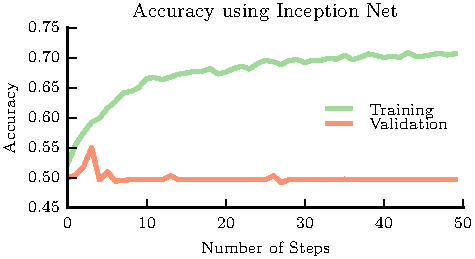
\includegraphics[width=0.75\columnwidth]{figs/inception_accuracy.pdf}
        \caption{Accuracy} \label{fig:accuracy}
        \end{subfigure}
    \begin{subfigure}[t]{0.49\textwidth}
        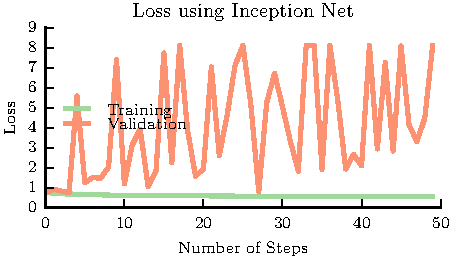
\includegraphics[width=0.75\columnwidth]{figs/inception_loss.pdf}
        \caption{Loss} \label{fig:loss}
    \end{subfigure}
\caption{The Loss and Accuracy across the Training and Validation Sets for our Inception Net} \label{fig:inception_results}
\end{figure*}

\begin{figure*}[t!]
    \begin{subfigure}[t]{0.49\textwidth}
        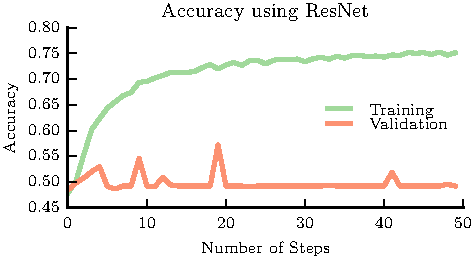
\includegraphics[width=0.75\columnwidth]{figs/balanced_resnet_accuracy.pdf}
        \caption{Accuracy} \label{fig:accuracy}
        \end{subfigure}
    \begin{subfigure}[t]{0.49\textwidth}
        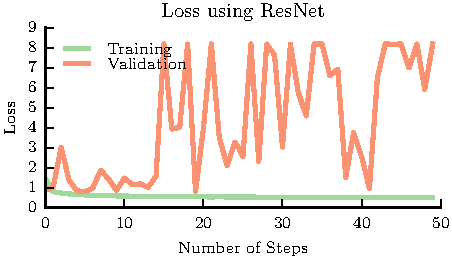
\includegraphics[width=0.75\columnwidth]{figs/balanced_resnet_loss.pdf}
        \caption{Loss} \label{fig:loss}
    \end{subfigure}
\caption{The Loss and Accuracy across the Training and Validation Sets for our ResNet using the balanced data set.} \label{fig:resnet_results}
\end{figure*}


\begin{figure}[t!]
    \centering
        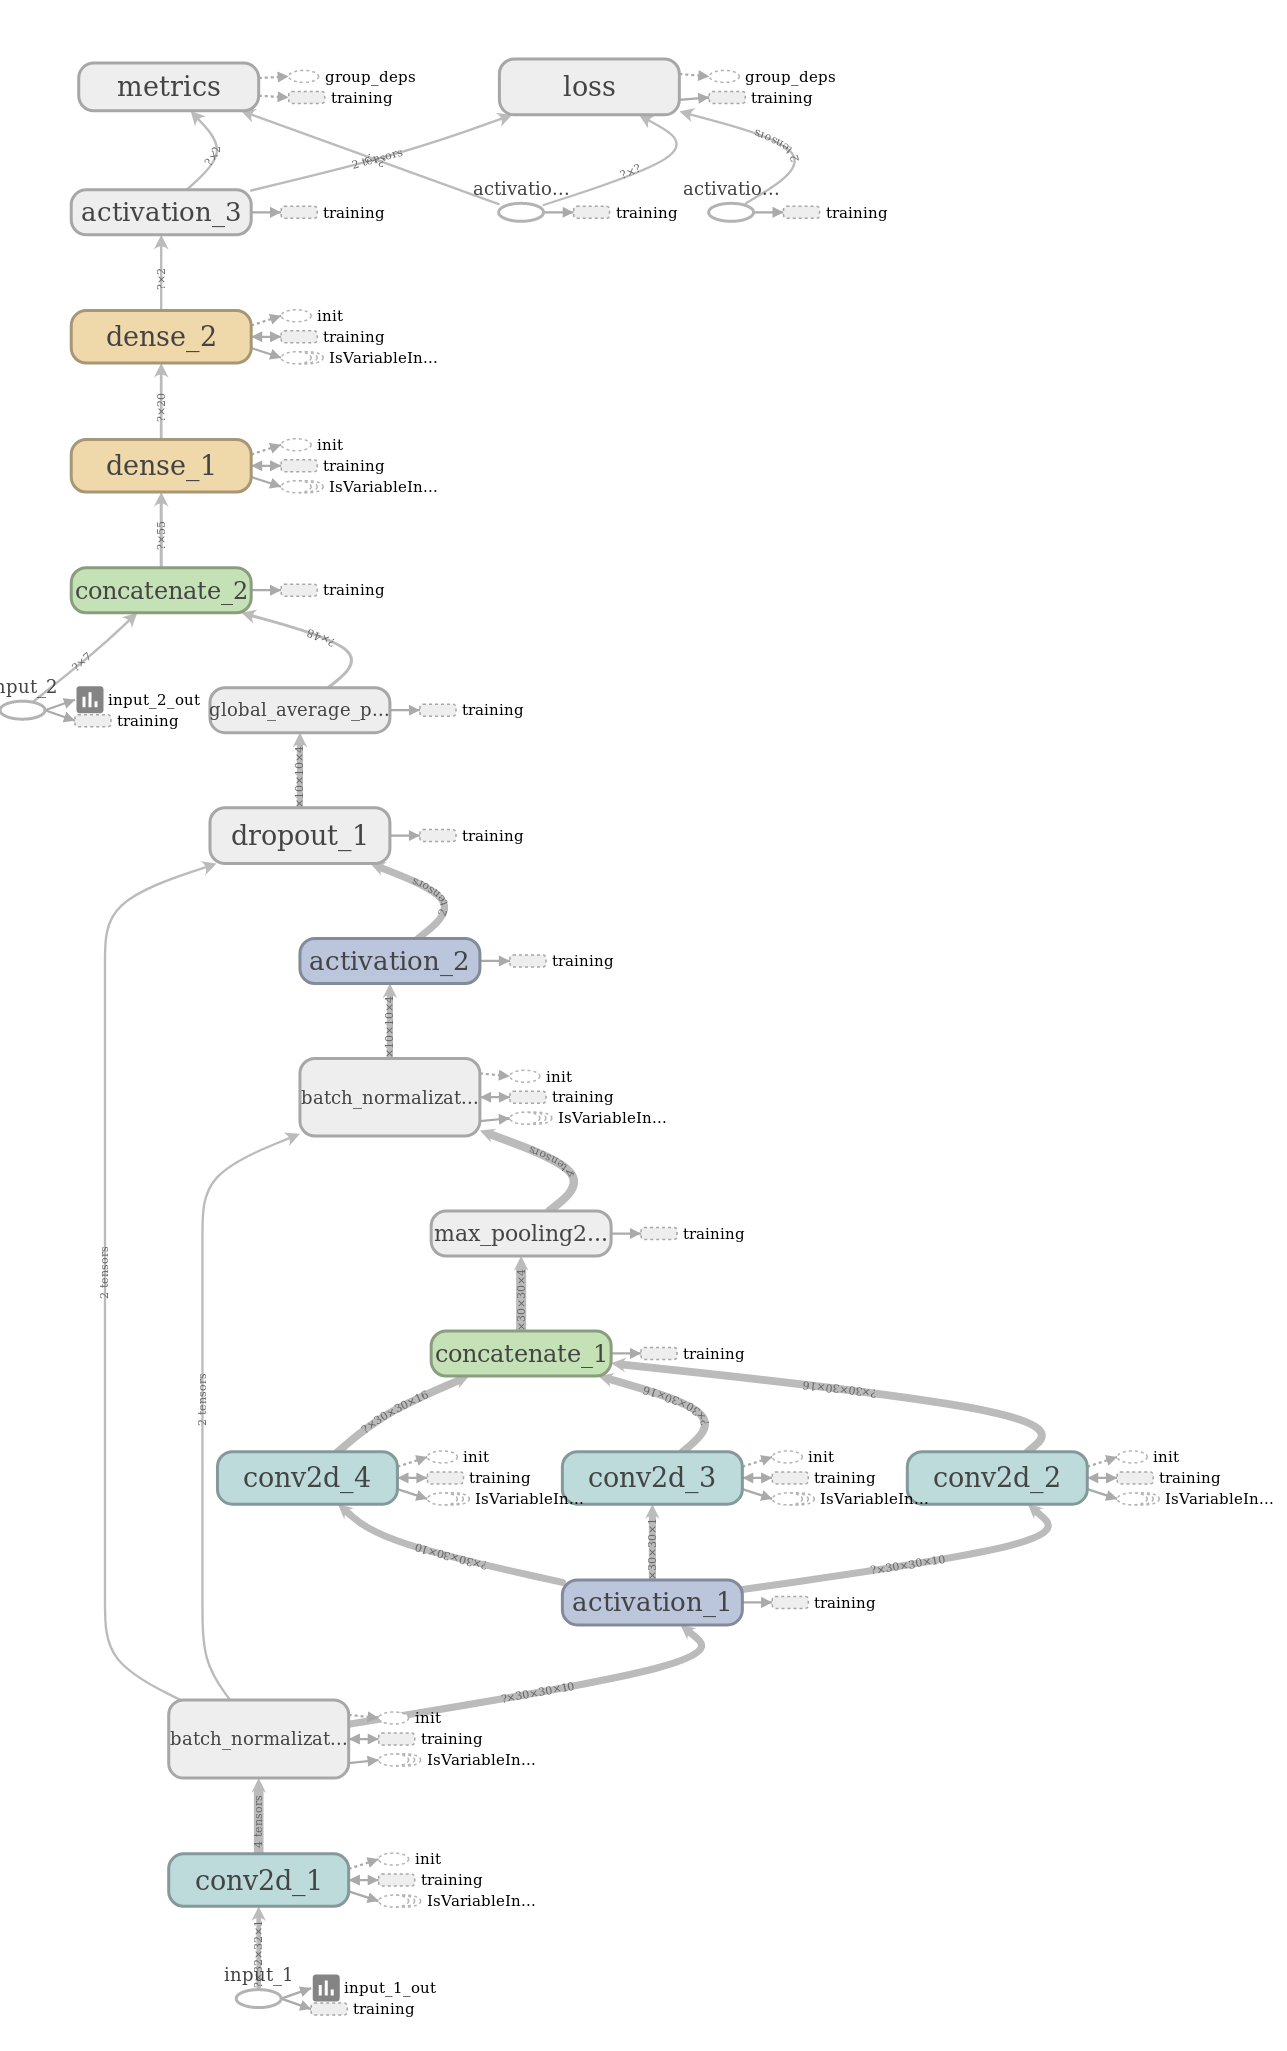
\includegraphics[width=0.7\columnwidth]{figs/inception_net.png}
    \caption{Network Structure of Inception Net} \label{fig:inception_net}
\end{figure}

\begin{figure}[t!]
    \centering
        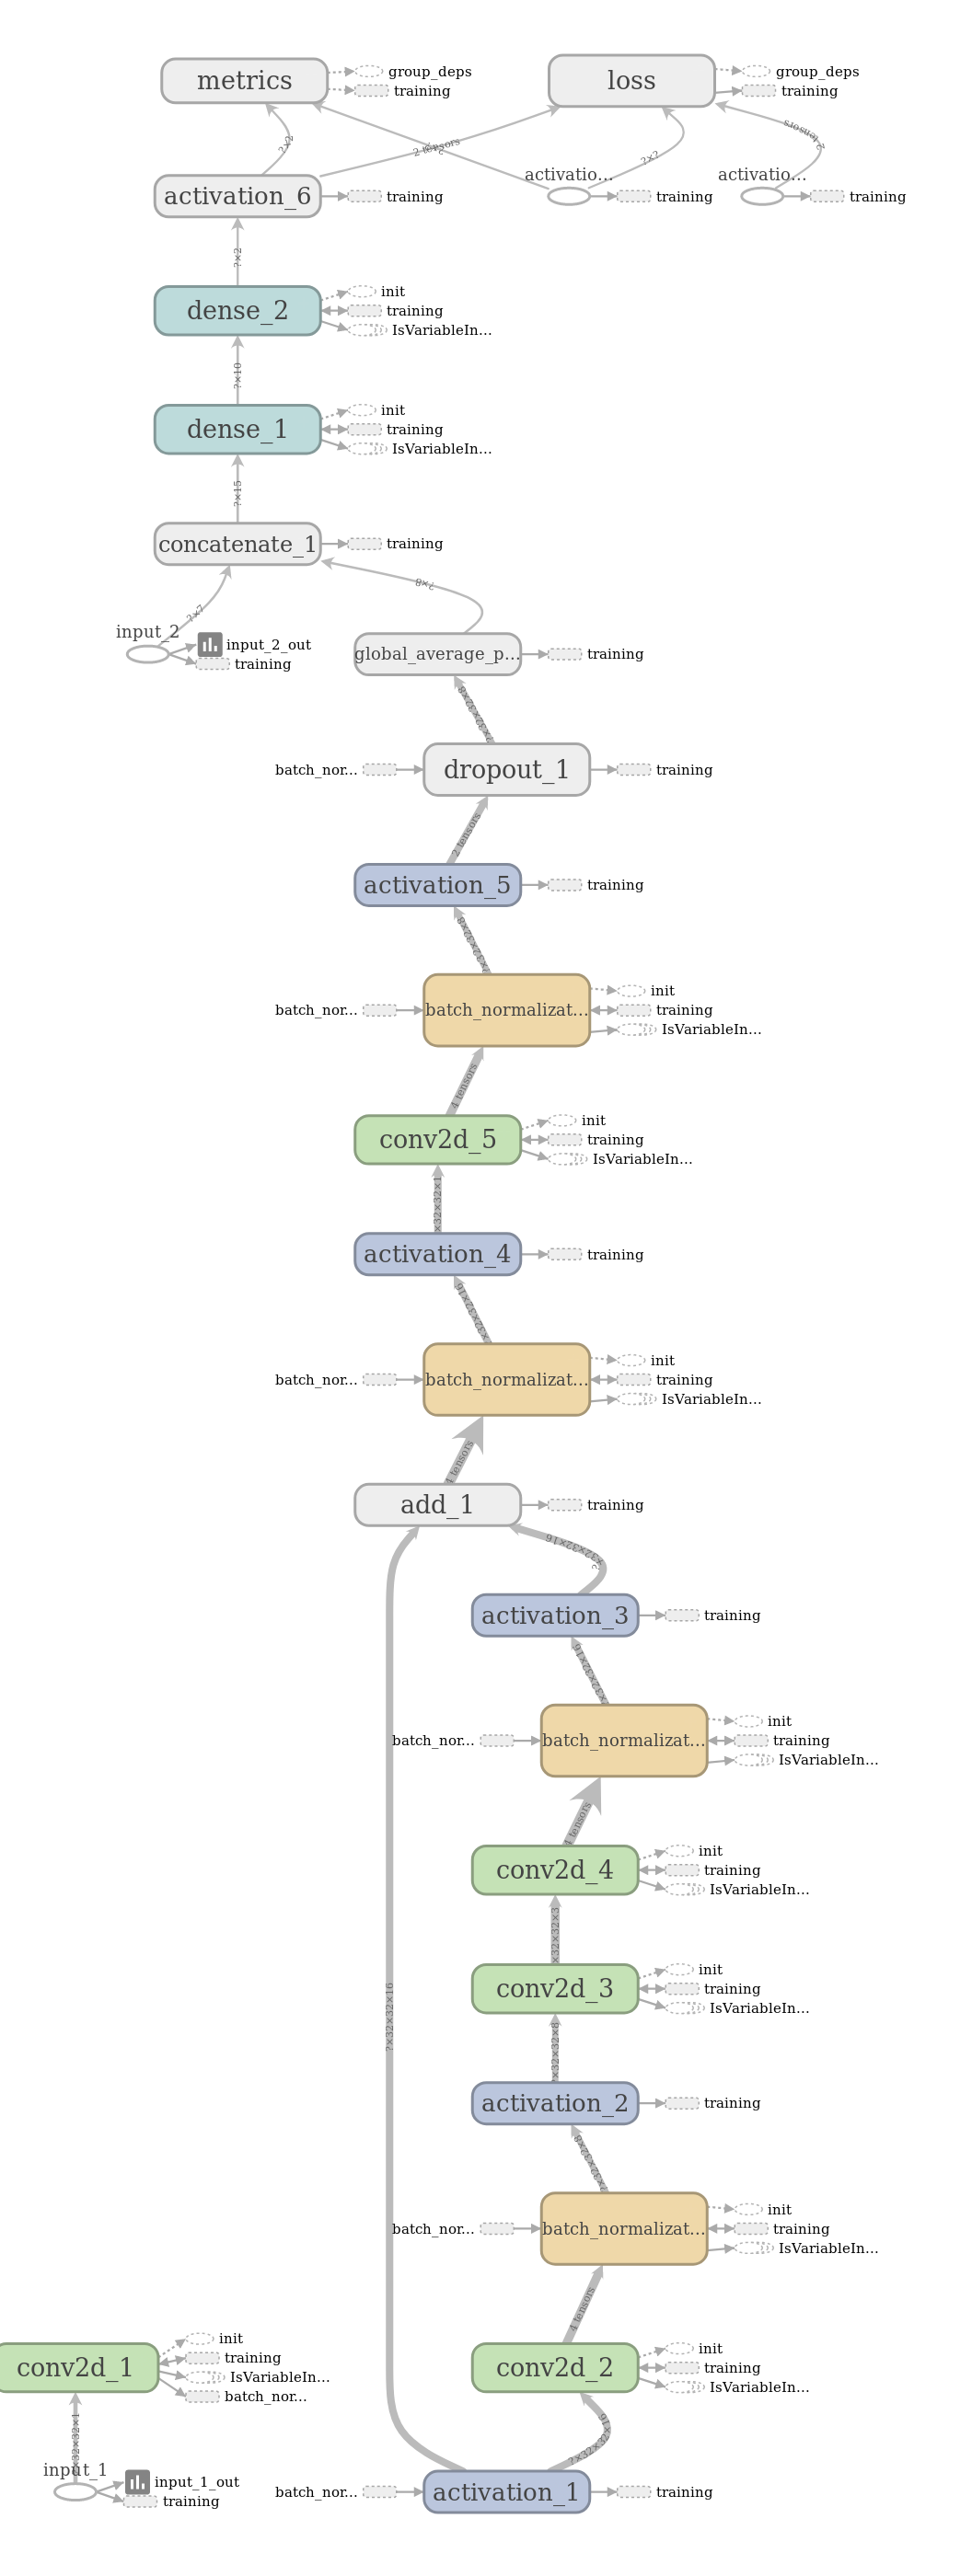
\includegraphics[width=0.7\columnwidth]{figs/balanced_resnet.png}
    \caption{Network Structure of ResNet} \label{fig:res_net}
\end{figure}

\section{Research Questions}
\label{sec:questions}

\subsection{Input Format}
One of the benefits of the Dex-Net data set is that it provides many features, allowing us to vary what we use as input to the network. 
We are and will continue to experiment with various inputs. 
Some inputs might be particularly informative but costly to collect when running the system on a real robot. 
Currently, the input format is a 32x32x1 depth map and a 1x7 pose vector. It is our intention to also use the representation used in the DexNet paper as soon as it becomes available.
This representation is as described in the Data Set section and shall serve as our baseline.. 

\subsection{Balancing Data Sets}
As mentioned previously, Dex-Net 2.0 contains approximately 20\% positive examples. 
This is not inherenely problematic given that the training and testing sets are drawn from the same distribution, with this same ratio.
However, by sampling subsets of our data set, we can achieve any positive-to-negative ratio and thus explore how changing this ratio effects accuracy. 
By doing this, we avoid a model to overfit and artificially think it is doing well by predicting ona class on all samples.  

\subsection{Data Set Size}
The Dex-net data set contains 6.7 million data points. 
For computational reasons, we are sampling a subset of these points. 
However, we can vary the size of this subset to compare the trade-off between the accuracy and the size of the training set. 
Deep learning models tend to require a rather large quantity of data depending the classification task that it is being learned and how complex the data is.
For now, since the data consists of just small 32x32x1 images and 1x7 vectors, and we learning a binary classification task, we reasoned that we could start by using a small subset of the 6.7 million data points
to produce a model of reasonable performance.

\subsection{Architecture Structure}
One of the largest sources of experimentation thus far and continuing forward is our choice of architecture. 
As our starting point, we produced an architecture that follows the concept of residual networks. This model consists of instead of learning a direct mapping of the input to the output, to learn ``residue'' over this input. Subsequently, we produced another architecture that follows the Inception model.
In this model, the concept applied was that each at each layer instead of doing one convolution layer we perform in parallel several convolution and pooling operations of different kernel sizes(1x1, 3x3, 5x5 convolutions, 3x3 max pooling), paired with dropout regularization with probability of 0.7.
The output of this parallel operations are concatenated on the depth dimension before being fed to the next layer. The idea behind this type of architecture is that, paired with regularization, the network could learn which mapping works best at each stage. In this iteration, we also trained the residual network
on balanced dataset with 0.7 dropout regularization. In addition, all networks have batch normalization after each convolution, to mitigate internal covariances shifts. Architecture details for each are shown in the figures. This are initial architectures and not final. As we keep training and modifying them accordingly, we will come up with the proper parameters using the validation and testing accuracy as our metric.

\section{Work Distribution}
\rhnote{give basically same thing as before}

\begin{comment}


Each object is paired with 2.5D point clouds, referred to as depth images, which are rendered with a variety of object and camera poses, where the camera intrinsics are known and used to center the depth image in a standardized fashion.
Each image is a black and white 32 by 32 pixel matrix. 

Therefore, we designed a simple Residual Network like the one shown in \figref{fig:network}. 
The idea is to pass the 32x32 depth maps through a ResNet with Batch Normalization to extract 1x8 features from it, and then these features are concatenated to the hand pose features that are passed to a fully connected layer that ouputs the likelihoods of each binary class. 
The training was carried in Keras~\cite{chollet2017keras}, using the RMSProp optimizer during 50 epochs with a batch size of 32 and 10\% of the dataset was used as Test. 
Given that we had a class imbalance of 1858 positive vs 8150 negatives in our datset subset, we assigned weights of 0.8 for positive and 0.2 for negative such that the underrepresented class could influnce training during each gradient descent step. 
This initial architecture did not work so well, however, since the error in the Test set was 81.0\%. 
If we observe the curves for loss and accuracy on Train and Validation during training in \figref{fig:loss} and \figref{fig:accuracy}, we can see that the network is overfitting.

\begin{figure*}[t!]
    \begin{subfigure}[t]{0.49\textwidth}
        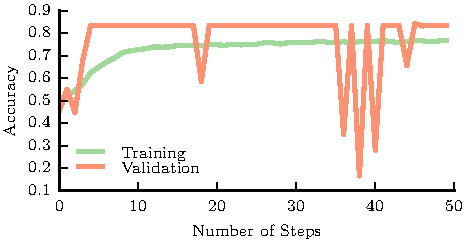
\includegraphics[width=0.99\columnwidth]{figs/accuracy.pdf}
        \caption{Accuracy} \label{fig:accuracy}
        \end{subfigure}
    \begin{subfigure}[t]{0.49\textwidth}
        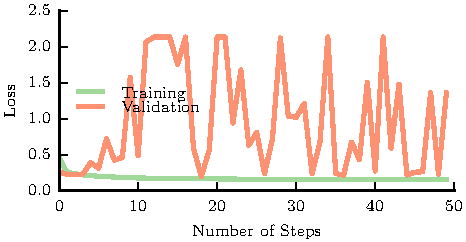
\includegraphics[width=0.99\columnwidth]{figs/loss.pdf}
        \caption{Loss} \label{fig:loss}
    \end{subfigure}
\caption{Initial Loss and Accuracy across the Training and Validation Sets} \label{fig:results}
\end{figure*}

\section{Division of Labor}

Rachel generated the training data from the DexNet data sets and set of the labeling mechanism. 
Sebastiani set up an environment in a AWS with GPUs, coded and trained initial Network In Network, Inception and ResNet based models in Keras/Tensorflow. 

\end{comment}

{\footnotesize
    \bibliographystyle{ieeetr}
\bibliography{../references}}

\end{document}
